\chapter{Análisis} \label{c.analisis}
\section{Análisis de riesgos completos} \label{c.analisis.riesgos}
A continuación se exponen las diferentes fases del análisis de riesgos de manera detallada: 

\begin{enumerate}

\item \textbf{Identificación de los riesgos}

Se han intentado considerar el máximo número de riesgos y se han clasificado en diferentes categorías:

%FASE 1: Identificación de los riesgos
\begin{itemize}

\item \textbf{Riesgos globales}
\begingroup
\renewcommand\arraystretch{1.3}

\begin{longtable}{l p{5cm} p{9cm}}
% header and footer information
\hline
\textbf{ID} & \textbf{Nombre} & \textbf{Explicación} \\
\hline
\endhead
\endfoot
RG\_1 & 
Plazos &
El proyecto no se finaliza para la convocatoria de junio, septiembre o diciembre.
 \\
RG\_2 & 
Fallo del equipo &
El equipo principal de desarrollo falla, se pierde o estropea. 
 \\
RG\_3 & 
Incorporación mercado &
El alumno se incorpora al mercado laboral durante el desarrollo del proyecto, a falta de varios meses de su finalización.
 \\
RG\_4 & 
Experiencia del alumno &
El alumno no dispone de los conocimientos y preparación suficiente para el desarrollo del proyecto. 
 \\
\hline
\caption{Riesgos globales del proyecto}\label{ries_glob}\\
\end{longtable}

\item \textbf{Riesgos tecnológicos}
\begin{longtable}{l p{5cm} p{9cm}}
% header and footer information
\hline
\textbf{ID} & \textbf{Nombre} & \textbf{Explicación} \\
\hline
\endhead
\endfoot
RT\_1 & 
Tecnología nueva &
Se trata de una tecnología nueva.
 \\
RT\_2 & 
Software no probado &
Se debe interactuar con software que no ha sido probado. 
 \\
RT\_3 & 
Interfaz especializada &
Es requerida una interfaz de usuario especializada.
 \\
RT\_4 & 
Componentes diferentes &
Se necesitan componentes de programa diferentes a los hasta ahora desarrollados.
 \\
RT\_5 & 
Rendimiento &
Se necesitan componentes de programa diferentes a los hasta ahora desarrollados.
 \\
RT\_6 & 
Inalcanzable &
Se necesitan componentes de programa diferentes a los hasta ahora desarrollados.
 \\
\hline
\caption{Riesgos tecnológicos del proyecto}\label{ries_tecno}\\
\end{longtable}

\item \textbf{Riesgos de alcance}
\begin{longtable}{l p{5cm} p{9cm}}
% header and footer information
\hline
\textbf{ID} & \textbf{Nombre} & \textbf{Explicación} \\
\hline
\endhead
\endfoot
RA\_1 & 
Tamaño estimado &
Tamaño estimado del proyecto
 \\
RA\_2 & 
Confianza en la estimación &
Confianza en la estimación
 \\
RA\_3 & 
Número de elementos &
Número de programas, archivos y transacciones
 \\
RA\_4 & 
Tamaño almacenamiento &
Tamaño de las bases de datos involucradas
 \\
RA\_5 & 
Número de usuarios &
Número de usuarios 
 \\
RA\_6 & 
Número de cambios &
Número de cambios en los requisitos
 \\
RA\_7 & 
Software reutilizado &
Cantidad de software utilizado
 \\
\hline
\caption{Riesgos de alcance del proyecto}\label{ries_alcan}\\
\end{longtable}

\item \textbf{Riesgos de entorno de desarrollo}
\begin{longtable}{l p{5cm} p{9cm}}
% header and footer information
\hline
\textbf{ID} & \textbf{Nombre} & \textbf{Explicación} \\
\hline
\endhead
\endfoot
RE\_1 & 
Gestión proyectos &
Hay herramientas de gestor de proyectos
 \\
RE\_2 & 
Gestión proceso desarrollo &
Hay herramientas de gestión del proceso de desarrollo
 \\
RE\_3 & 
Análisis y diseño &
Se usan métodos y herramientas específicas para el análisis y diseño 
 \\
RE\_4 & 
Generadores de código &
Hay generadores de código apropiados para la aplicación
 \\
RE\_5 & 
Pruebas &
Hay herramientas de pruebas apropiadas
 \\
RE\_6 & 
Gestión de configuración &
Hay herramientas de gestión de configuración apropiadas
 \\
RE\_7 & 
Base de datos  &
Se hace uso de una base de datos o repositorio centralizado
 \\
RE\_8 & 
Integración &
Están todas las herramientas de desarrollo integradas
 \\
RE\_9 & 
Formación &
Se ha proporcionado formación a todos los miembros del equipo de desarrollo
 \\
RE\_10 & 
Expertos &
Hay expertos a los cuales solicitar ayuda acerca de las herramientas
 \\
RE\_11 & 
Ayuda online &
Hay ayuda en línea y documentación disponible
 \\
RE\_12 & 
Diseño arquitectónico &
Se utiliza un  método específico para el diseño arquitectónico y de datos
 \\
RE\_13 & 
Métricas de calidad &
Se disponen métricas de calidad para todos los proyectos de software
 \\
RE\_14 & 
Métricas de productividad &
Se disponen de métricas de productividad
\\
\hline
\caption{Riesgos de entorno de desarrollo del proyecto}\label{ries_entorno}\\
\end{longtable}

\endgroup

\end{itemize}

\item \textbf{Análisis del riesgo} \par

Para esta fase se han empleado los tres medidores del riesgo: la probabilidad, el impacto y la aceptación: 

%FASE 2: Análisis del riesgo - INTRODUCCION
\begin{itemize}

\item{\textbf{Tabla para estimar la probabilidad de un riesgo:}}
\begingroup
\renewcommand\arraystretch{1.3}
\begin{longtable}{l p{13cm}}
% header and footer information
\hline
\textbf{Valor} & \textbf{Descripción} \\
\hline
\endhead
\endfoot
Bajo (1) & 
La amenaza se materializa a lo sumo una vez cada año. 
 \\
Medio (2) & 
La amenaza se materializa a lo sumo una vez cada mes.
 \\
Alto (3) & 
La amenaza se materializa a lo sumo una vez cada semana.
 \\
\hline
\caption{Probabilidad de un riesgo}\label{prob_riesgo}\\
\end{longtable}

\item{\textbf{Tabla para estimar el impacto de un riesgo:}}
\begin{longtable}{l p{13cm}}
% header and footer information
\hline
\textbf{Valor} & \textbf{Descripción} \\
\hline
\endhead
\endfoot
Bajo (1) & 
El daño derivado de la materialización de la amenaza no tiene consecuencias relevantes para la consecución de los objetivos.  
 \\
Medio (2) & 
El daño derivado de la materialización de la amenaza tiene consecuencias reseñables para la consecución de los objetivos.
 \\
Alto (3) & 
El daño derivado de la materialización de la amenaza tiene consecuencias graves reseñables para la consecución de los objetivos.
 \\
\hline
\caption{Impacto de un riesgo}\label{impacto_riesgo}\\
\end{longtable}

\item{\textbf{Tabla para estimar la aceptación de un riesgo:}}


\begin{longtable}{l p{13cm}}
% header and footer information
\hline
\textbf{Valor} & \textbf{Descripción} \\
\hline
\endhead
\endfoot
Riesgo $\leq$ & 
La organización considera el riesgo poco reseñable. 
 \\
Riesgo $\geq$ 4 & 
La organización considera el riesgo reseñable y debe proceder a su tratamiento.
 \\
\hline
\caption{Aceptación de un riesgo}\label{aceptacion_riesgo}\\
\end{longtable}

\endgroup
\end{itemize}
\par La aceptación es una medida delimitadora que define aquellos riesgos que son considerados aceptables y aquellos ante los que se deben tomar medidas. Para esta medida se ha establecido un criterio de aceptación de 4. Cualquier riesgo cuyo valor sea menor que 4 se considera aceptable y por tanto un riesgo poco reseñable, mientras que aquellos que se encuentran por encima de 4 se consideran reseñables y se debe proceder a su tratamiento. 
\par
El cálculo de la gravedad del riesgo y su aceptación se realiza de la siguiente manera: se multiplica la probabilidad por el impacto, y si dicho valor excede el límite del criterio de aceptación, el riesgo se considera reseñable. 
A continuación, en base a las métricas anteriores, se especifican los riesgos de la fase 1 en las mismas categorías iniciales. Se resaltan en rojo aquellos riesgos cuya aceptación supera el 4.

%FASE 2: Análisis del riesgo - TABLAS
\begin{itemize}

\item \textbf{Riesgos globales}
\begingroup
\renewcommand\arraystretch{1.3}

\begin{longtable}{l p{5cm} ccc}
% header and footer information
\hline
\textbf{ID} & \textbf{Nombre} & \textbf{Probabilidad} & \textbf{Impacto} & \textbf{Riesgo} \\
\hline
\endhead
\endfoot
\textbf{RG\_1} & 
\textbf{Plazos} &
\textbf{2} &
\textbf{3} &
\textbf{6} 
 \\
RG\_2 & 
Fallo del equipo &
1 &
3 &
3 
 \\
RG\_3 & 
Incorporación mercado &
1 &
2 &
2 
 \\
RG\_4 & 
Experiencia del alumno &
2 &
2 &
4 
 \\
\hline
\caption{Valoración riesgos globales del proyecto}\label{ries_glob_valoracion}\\
\end{longtable}

\item \textbf{Riesgos tecnológicos}
\begin{longtable}{l p{5cm} ccc}
% header and footer information
\hline
\textbf{ID} & \textbf{Nombre} & \textbf{Probabilidad} & \textbf{Impacto} & \textbf{Riesgo} \\
\hline
\endhead
\endfoot
RT\_1 & 
Tecnología nueva &
3 &
1 &
3 
 \\
\textbf{RT\_2} & 
\textbf{Software no probado} &
\textbf{2} &
\textbf{3} &
\textbf{6} 
 \\
RT\_3 & 
Interfaz especializada &
1 &
1 &
1 
 \\
RT\_4 & 
Componentes diferentes &
3 &
1 &
3 
 \\
RT\_5 & 
Rendimiento &
2 &
2 &
4 
 \\
\textbf{RT\_6} & 
\textbf{Inalcanzable} &
\textbf{2} &
\textbf{3} &
\textbf{6} 
 \\
\hline
\caption{Valoración riesgos tecnológicos del proyecto}\label{ries_tecno_valoracion}\\
\end{longtable}

\item \textbf{Riesgos de alcance}
\begin{longtable}{l p{5cm} ccc}
% header and footer information
\hline
\textbf{ID} & \textbf{Nombre} & \textbf{Probabilidad} & \textbf{Impacto} & \textbf{Riesgo} \\
\hline
\endhead
\endfoot
\textbf{RA\_1} & 
\textbf{Tamaño estimado} &
\textbf{2} &
\textbf{3} &
\textbf{6} 
 \\
RA\_2 & 
Confianza en la estimación &
2 &
2 &
4 
 \\
\textbf{RA\_3} & 
\textbf{Número de elementos} &
\textbf{2} &
\textbf{3} &
\textbf{6} 
 \\
RA\_4 & 
Tamaño almacenamiento &
1 &
3 &
3 
 \\
RA\_5 & 
Número de usuarios &
1 &
3 &
3 
 \\
\textbf{RA\_6} & 
\textbf{Número de cambios} &
\textbf{2} &
\textbf{3} &
\textbf{6} 
 \\
RA\_7 & 
Software reutilizado &
1 &
1 &
1 
 \\
\hline
\caption{Riesgos de alcance del proyecto}\label{ries_alcan}\\
\end{longtable}

\item \textbf{Riesgos de entorno de desarrollo}
\begin{longtable}{l p{5cm} ccc}
% header and footer information
\hline
\textbf{ID} & \textbf{Nombre} & \textbf{Probabilidad} & \textbf{Impacto} & \textbf{Riesgo} \\
\hline
\endhead
\endfoot
RE\_1 & 
Gestión proyectos &
1 &
1 &
1 
 \\
RE\_2 & 
Gestión proceso desarrollo &
1 &
1 &
1 
 \\
RE\_3 & 
Análisis y diseño &
1 &
2 &
2 
 \\
RE\_4 & 
Generadores de código &
1 &
1 &
1 
 \\
RE\_5 & 
Pruebas &
2 &
2 &
4 
 \\
RE\_6 & 
Gestión de configuración &
2 &
2 &
4 
 \\
RE\_7 & 
Base de datos  &
1 &
3 &
3 
 \\
RE\_8 & 
Integración &
1 &
1 &
1 
 \\
\textbf{RE\_9} & 
\textbf{Formación} &
\textbf{2} &
\textbf{3} &
\textbf{6} 
 \\
RE\_10 & 
Expertos &
2 &
1 &
2 
 \\
RE\_11 & 
Ayuda online &
2 &
2 &
4 
 \\
RE\_12 & 
Diseño arquitectónico &
2 &
1 &
2 
 \\
RE\_13 & 
Métricas de calidad &
3 &
1 &
3 
 \\
RE\_14 & 
Métricas de productividad &
3 &
1 &
3 
\\
\hline
\caption{Valoración de los riesgos de entorno de desarrollo del proyecto}\label{ries_entorno_valoracion}\\
\end{longtable}

\endgroup

\end{itemize}

\item \textbf{Priorización de riesgos} \par
Esta fase incluye todos los riesgos, ordenados de mayor a menor severidad. Se resaltan en rojo los riesgos que habrá que considerar en un plan de defensa estratégico posterior:


\begingroup
\renewcommand\arraystretch{1.3}

\begin{longtable}{l p{5cm} c}
% header and footer information
\hline
\textbf{ID} & \textbf{Nombre} & \textbf{Riesgo} \\
\hline
\endhead
\endfoot
\textbf{RG\_1} & 
\textbf{Plazos} &
\textbf{6} 
 \\
\textbf{RT\_2} & 
\textbf{Software no probado} &
\textbf{6} 
 \\
\textbf{RT\_6} & 
\textbf{Inalcanzable} &
\textbf{6} 
 \\
\textbf{RA\_1} & 
\textbf{Tamaño estimado} &
\textbf{6} 
 \\
\textbf{RA\_6} & 
\textbf{Número de cambios} &
\textbf{6} 
 \\
\textbf{RE\_9} & 
\textbf{Formación} &
\textbf{6} 
 \\
 
RT\_5 & 
Rendimiento &
4 
 \\
RA\_2 & 
Confianza en la estimación &
4 
 \\
RE\_5 & 
Pruebas &
4 
 \\
RE\_11 & 
Ayuda online &
4 
 \\
RG\_2 & 
Fallo del equipo &
3 
 \\
RT\_1 & 
Tecnología nueva &
3 
 \\
RT\_4 & 
Componentes diferentes &
3 
 \\
RA\_4 & 
Tamaño almacenamiento &
3 
 \\
RA\_5 & 
Número de usuarios &
3 
 \\
RE\_7 & 
Base de datos &
3 
 \\
RE\_13 & 
Métricas de calidad &
3 
 \\
RE\_14 & 
Métricas de productividad &
3 
 \\
RG\_3 & 
Incorporación mercado &
2 
 \\
RE\_3 & 
Análisis y diseño &
2 
 \\
RE\_10 & 
Expertos &
2 
 \\
RE\_12 & 
Diseño arquitectónico &
2 
 \\
RT\_3 & 
Interfaz especializada &
1 
 \\
RT\_7 & 
Software reutilizado &
1 
 \\
RE\_1 & 
Gestión proyectos &
1 
 \\
RE\_2 & 
Gestión proceso desarrollo &
1 
 \\
RE\_4 & 
Generadores de código &
1 
 \\
RE\_8 & 
Integración &
1 
 \\
\hline
\caption{Priorización de riesgos del proyecto}\label{prioriz_riesg}\\
\end{longtable}

\endgroup
Como se puede apreciar, hay 6 riesgos cuyo factor de gravedad es preocupante y deben ser tratados acordemente: 
\begin{enumerate}
\item RG\_1. Riesgo global “Plazos”. Tiene que ver con el hecho de no acabar el proyecto dentro de los plazos establecidos para su defensa. Hay 2 fechas recomendables para su defensa, la primera en Junio de 2017 y la segunda en Septiembre de 2017. No obstante, se dispone de otra oportunidad en Diciembre de 2017, aunque sería la menos recomendable dado que supondría el retraso de la defensa y con ello la dificultad del estudiante de realizar otras actividades mientras tanto. A partir de Diciembre, la consecuencia sería volver a matricularse en el proyecto y aportar las tasas de la matrícula por segunda vez.
\item RT\_2. Riesgo de tecnologías “Software no probado”. Tiene que ver con la probabilidad de usar en el proyecto software que previamente no ha sido probado y pueda fallar. Obtuvo una valoración de gravedad de 6/6 puesto que si bien es cierto que todas las tecnologías han sido probadas individualmente y se sabe que funcionan bien, el proceso en su conjunto no ha sido probado. No se sabe si es viable o no.  
\item RT\_6. Riesgo de tecnologías “Inalcanzable”. Relacionado con el hecho de que el proyecto puede tener como conclusión un resultado negativo; Al tratarse de un trabajo de investigación, el resultado puede ser que no se ha logrado la integración deseada.
\item RA\_1. Riesgo de alcance “Tamaño estimado”. Tiene que ver con el hecho de que el proyecto resulte mucho más grande de lo estimado inicialmente, y por diferentes circunstancias no se llegue a finalizar.
\item RA\_6. Riesgo de alcance “Número de cambios”. Otro riesgo es el hecho de que los requisitos cambien constantemente, bien porque los clientes lo solicitan bien porque las propias tecnologías lo imponen. 
\item RE\_9. Riesgo de entorno de desarrollo “Formación”. Este riesgo trata con el hecho de que el alumno disponga de la formación necesaria y suficiente para lograr los objetivos propuestos.
\end{enumerate}

\item \textbf{Planificación de la gestión de riesgos} \par
En esta fase se recogen las conclusiones mitigadoras acerca de los riesgos "preocupantes" del proyecto, en relación a su factor de gravedad: 

\begin{enumerate}
\item RG\_1: Plazos - Como medida mitigante, el alumno deberá dedicar un horario de jornada completa a la realización del proyecto durante el verano del año 2017. 
\item RT\_2: Software no probado - La contrapartida y defensa de este riesgo es desarrollar o experimentar primero con una prueba de concepto para validar que las tecnologías en su conjunto funcionen correctamente. 
\item RT\_6: Inalcanzable - La mitigación este riesgo está ligada al anterior. Por lo tanto, primero se hará una prueba de concepto para demostrar si las tecnologías empleadas se pueden usar en conjunto.
\item RA\_1: Tamaño estimado - La solución desde un principio debe definir bien el alcance y determinar aquellas cosas que formarán parte de la solución y aquellas que no lo harán. 
\item RA\_6: Número de cambios - El alumno y el profesor deben acordar al principio unos requisitos fijos que no podrán ser modificables, en conjunto con el hecho de definir claramente el alcance de la solución.
\item RE\_9: Formación - Para mitigar este riesgo, el alumno debe estar en constante aprendizaje, utilizando los manuales y tutoriales de las diferentes herramientas de las que va a hacer uso durante el proyecto. Además, el alumno tendrá a su disposición al director del proyecto para consultar dudas y a los diferentes foros tecnológicos de Internet. 
\end{enumerate}
\end{enumerate}

\section{Análisis de diseños alternativos} \label{c.analisis.disenyos}

Al igual que los requisitos, el diseño de la solución también ha sufrido constantes cambios. Inicialmente la propuesta de trazabilidad de la solución es la que se puede observar en la figura 1. \par

\begin{figure}[H]
    \centering
    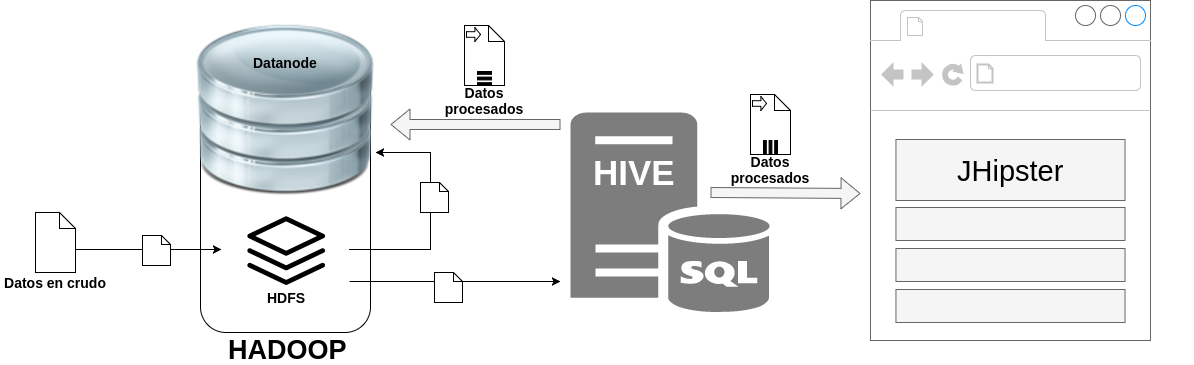
\includegraphics[width=1\textwidth,height=5.5cm]{Imagenes/Dis_Fig_1}
    \caption{Diseño primitivo del sistema.}
    \label{fig:dis_1_sist}
\end{figure}
\par


Como se puede observar, inicialmente el concepto giraba alrededor de las tres tecnologías core: Hadoop, Hive y JHipster. No se tuvo en consideración otras herramientas puesto que se pensaba que era suficiente para resolver el problema. Los datos en crudo, extraídos de la web del magrama o de otras fuentes heterogéneas, serían almacenados en Hadoop, en un nodo local mediante el sistema de ficheros HDFS, y posteriormente sería HIVE el encargado de procesarlos en su totalidad hasta conseguir almacenarlos en un esquema común. Además, la misma “base de datos” de Hive funcionaría como base de datos para la aplicación desarrollada con JHipster, sirviendo en todo momento ese esquema único para la visualización del mismo en un navegador web. Este diseño, conceptualmente fue la solución ideal para el problema planteado; no obstante, debido a que JHipster no ofrece soporte para cambiar la base de datos con la que se construye la aplicación y mucho menos soporte para Hive o Hadoop, tras muchos intentos frustrados de conseguir esta conectividad directa, se optó por una solución diferente, alejada de este diseño ideal pero rebelde, en contra de los paradigmas de programación que JHipster impone. La alternativa a este diseño que dió resultados y eliminó complicaciones fue la que se observa en la figura 2. \par


\begin{figure}[H]
    \centering
    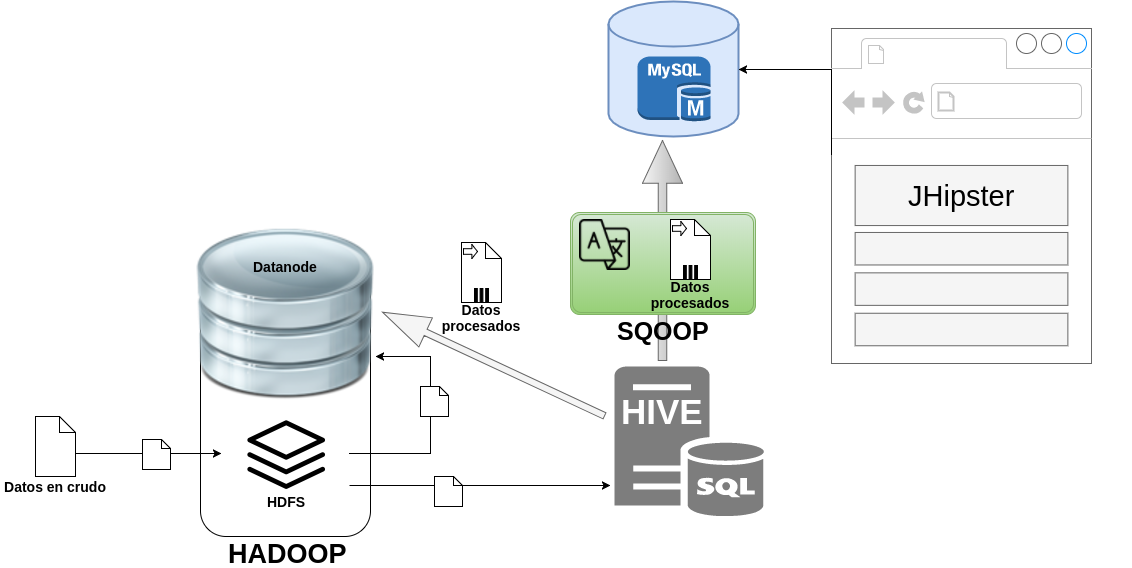
\includegraphics[width=1\textwidth,height=8cm]{Imagenes/Dis_Fig_2}
    \caption{Segunda iteración del diseño del sistema.}
    \label{fig:dis_2_sist}
\end{figure}
\par


En la segunda fase del diseño, se observa la evolución de la idea, condicionada por los problemas anteriormente mencionados. En primer lugar, se conservó la base de datos nativa de JHipster, en este caso una base de datos MySQL convencional. En ella se almacenaria únicamente la estructura final del esquema unificado, con los datos finales. Dichos datos tendrían que ser pasados desde Hive mediante una herramienta de transformación y transporte de datos. En este caso se usó Sqoop, una herramienta gratuita que permite transportar los datos desde Hive a MySQL, puesto que ofrece soporte tanto para Hadoop, HDFS y Hive como para MySQL. \par
Una vez resuelto el problema de la visualización de los datos, lo próximo que se detectó fue esa necesidad de procesamiento de los datos en crudo antes de incluso exponerlos como un esquema relacional en Hive. Para eso, lo mejor era hacer uso de algún programa de procesado de ficheros y una de las mejores opciones aparentes era Pentaho, un programa completo de transformación de ficheros. Pentaho venía con soporte para Hadoop y HDFS, por lo que gracias a eso se pudo trabajar con ficheros directamente extraídos de Hadoop, y almacenarlos directamente en Hadoop. Los cambios se pueden observar en la figura 3. \par


\begin{figure}[H]
    \centering
    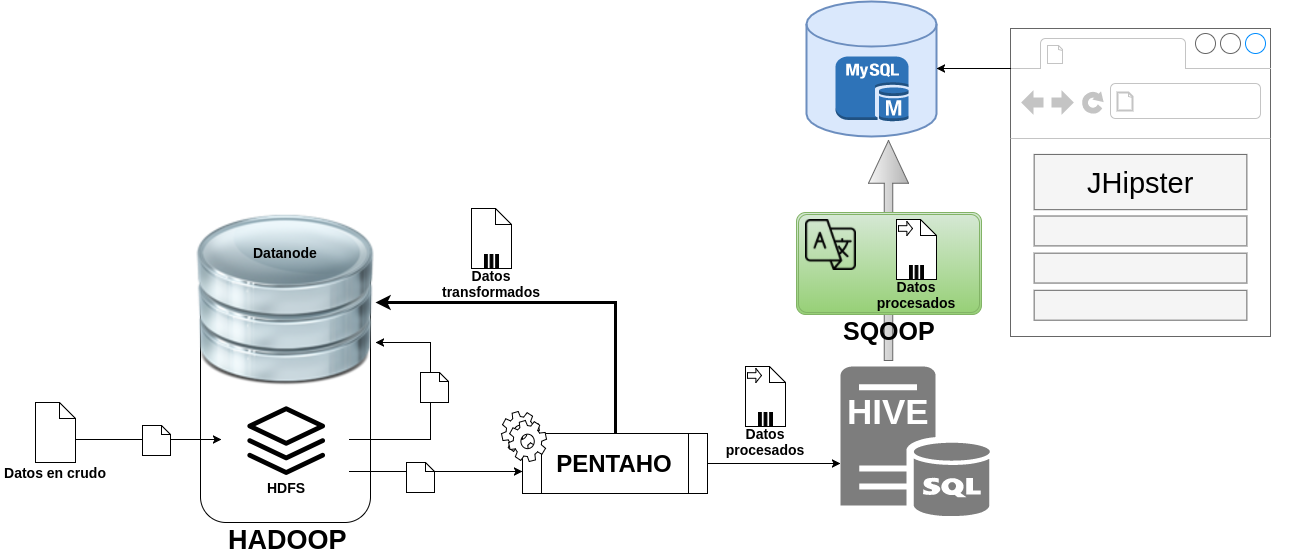
\includegraphics[width=1\textwidth,height=7cm]{Imagenes/Dis_Fig_3}
    \caption{Tercera iteración del diseño del sistema.}
    \label{fig:dis_2_sist}
\end{figure}
\par


INACABADO

